% \textbf{Social Recommendations:} Software engineering is a social activity~\cite{ahmadi2008survey}, and this principle refers to prioritizing community and social aspects of programming when generating recommendations to developers.  In our results, we found most participants turn to social media and public online resources to learn about new tools. For example, one participant mentioned ``I sorta want to hear about it where I hear about other programming tools. I want to see it on Twitter... It's good when these people have taken the time to talk about it" (P1). Furthermore, Begel et al suggest social media has impacted how software engineers communicate, gain knowledge, and share information~\cite{begel2010social}. An example of social recommendations includes ToolBox, which offers \textit{community sensitive} recommendations for Unix commands based on similar actions by users on a shared network~\cite{ToolBox}. We believe finding ways to integrate social influence and popular opinion into automated recommendations will encourage developer adoption.


% \textbf{Actionable Recommendation:} Actionability refers to the ease with which users can act on recommendations. In nudge theory, research suggests actionability is a key concept for encouraging humans to make better decisions. A simple nudge is to make target behaviors easy to apply because ``many people will take whatever option requires the least effort, or the path of least resistance"~\cite[p.~85]{sunstein2008nudge}. In our user study, we found developers preferred the suggested changes recommendation because it's ``easier to submit" (P5) and has ``pretty neat integration" (P1). In software engineering research, Heckman and colleagues examined the concept of actionability through static analysis notifications in AAITs (actionable alert identification techniques) to help developers identify and resolve defects in code~\cite{HECKMAN2011363}. We propose making automated development tool recommendations actionable will encourage the adoption from developers.

% \textbf{Receptive Choice Architectures:} Research shows user receptiveness important for making effective recommendations. For example, the \peer study shows that receptiveness significantly impacts the outcome of tool recommendations~\cite{Interactions}. Additionally, Fogg suggests receptive audiences are important for creating persuasive technologies~\cite{fogg2009persuasive}. To leverage nudge theory and choice architecture to improve receptiveness, we suggest emphasizing the locality of recommendations. For contextualizing this concept into design implications, we divide locality into two subcategories: \textit{spatial} and \textit{temporal} locality.



\section{Developer Recommendation Choice Architectures}

The preliminary results show that receptiveness and development context are required for effective developer recommendations. To improve these recommendations, I present the following \textbf{\em developer recommendation choice architectures} to design and frame decisions for software engineers based on nudge theory and software engineering literature: \textbf{actionability}, \textbf{feedback}, and \textbf{locality}. We aim to show that incorporating these choice architectures into developer recommendations can improve the decision-making of software engineers.

\subsection{Actionability} Actionability refers to the ease with which users can act on recommendations. In nudge theory, research suggests actionability is a key concept for encouraging humans to make better decisions. A simple nudge is to make target behaviors easy to apply because ``many people will take whatever option requires the least effort, or the path of least resistance"~\cite[p.~85]{sunstein2008nudge}. For example, one simple nudge to improve the actionability of recommendations is to change the default rule. Madrian and Shea implemented this nudge to encourage employees to enroll in retirement plans. By having users opt-out of 401k plans instead of automatically opting in, they discovered that this improved money saving behaviors and encouraged more employees to join and enroll sooner, with 98\% of new employees selecting a plan within 36 months~\cite{madrian2001power}. In this instance, the easiest option to adopt was the default selection. Software engineering research also shows actionability is important to developers. Heckman and colleagues examined the concept of actionability through static analysis notifications in AAITs (actionable alert identification techniques) to help developers identify and resolve defects in code~\cite{HECKMAN2011363}. We propose making automated development tool recommendations actionable will encourage the adoption from developers.

\subsection{Feedback} Sunstein and Thaler note that ``the best way to help Humans improve their performance is to provide feedback" and ``choices can be improved with better and simpler information"~\cite[p.~92,~204]{sunstein2008nudge}. For example, most people order familiar and repeated meals at fast food restaurants, however nudges such as providing information on the amount of calories in food and feedback on recommended daily caloric intake encouraged consumers to purchase unfamiliar and healthier meals~\cite{Wisdom2010Healthy}. In this case, feedback refers to information provided to impact developer behavior.
Software engineering researchers also show that feedback to developers is important. For instance, Barik and colleagues examined the impact of compiler error message feedback on how developers resolved problems~\cite{barik2018should}. Furthermore, Cerezo and colleagues also suggest that user-driven communication can improve the perception of chatbots as opposed to single-purpose bot-driven techniques~\cite{cerezo2019building}. To improve the effectiveness of automated recommendations to software engineers, we believe providing useful information and feedback will improve the likelihood developers adopt useful behaviors.

\subsection{Locality} Locality refers to the setting of recommendations in the context of developers completing programming tasks. To describe the locality of developer recommendations, we divide this concept into two subcategories: \textit{spatial} and \textit{temporal} locality.

\subsubsection{Spatial:} Spatial locality refers to the location where recommendations are made. Nudge theory suggests that the location of recommendations matters when encouraging people to adopt useful behaviors. For example, Hanks found that changing the location of vegetables, fruits, etc. in a high school cafeteria increased the purchase and consumption of healthier foods by students~\cite{Hanks2012Lunchroom}. Research shows that the location of recommendations matters to developers and they prefer notifications are placed in convenient locations. Johnson et al. reported that developers felt inconvenienced leaving their normal coding environment to use development tools~\cite{Johnson2013Why}. Similarly, de Alwis and colleagues found that the inability to locate navigation and displays made developers feel disoriented in the Eclipse IDE~\cite{de2006using}. In our prior work, we developed an Eclipse code navigation plugin, \textsc{Flower}, which was developed with \textit{in situ} navigation design principles to avoid developer disorientation and switching between views. In our evaluation of this tool, we found that the location of suggestions within the IDE and led to increased efficiency with branchless navigation and positive responses from participants on the user interface~\cite{Flower}. In designing choice architectures for recommendations to developers, we propose making automated suggestions to developers in familiar and convenient locations to target user receptivity and encourage adoption.

% Sunstein and Thaler categorize ``hot" and ``cold" states and note that humans are more likely to make certain decisions during hot times~\cite[p.~41]{sunstein2008nudge}. For example, a study found that simply asking people if they intend to purchase a new car within the next six months actually increased purchase rates by 35\%~\cite{morwitz1993intent}.

\subsubsection{Temporal:} Temporal locality refers to the timing of when recommendations are made to users. In nudge theory, timing plays a major role in impacting human decision-making. For example, an effective nudge for farmers in Kenya was to change the time of year for fertilizer discounts. This encouraged them to make purchases earlier in time to improve the harvest of crops~\cite{duflo2011nudging}. Software engineering research also shows that behavioral recommendation timing is important in software engineering. For example, Distefano examined configuring static analysis tools to run at \textit{diff time}, or on patches submitted by developers to review before merging into the code base, and found that this increased the fix rate of reported bugs up to 70\% compared to nearly 0\% for times outside the development workflow, such as assigning bug lists to developers from overnight builds~\cite{Distefano2019Facebook}. To incorporate nudges into software engineering recommendations and choice architecture designs, we propose developing automated systems that make timely suggestions to programmers within their workflow to increase their desire to adopt useful behaviors and practices.

\newpage

%------- nothing below ----------%

% \begin{table}[H]
% \centering
% \begin{tabular}{lll} \hline
%   \textsc{Nudge} & \textsc{Failure} & \textsc{Example} \\ \hline
%  \textbf{Location} &  Familiarity & \textit{automated pull requests} \\
%  \textbf{Timing} &  Familiarity & \textit{automated pull requests} \\
%  \textbf{Feedback} & Social Context  & \textit{better feedback} \\
%  \textbf{Actionability} & Developer Workflow & \textit{automated pull requests} \\ 
%   & Desire & \\ \hline
% \end{tabular}
% \caption{Nudges for Software Engineering Recommendations}
% \label{tab:approach}
% \end{table}

% \paragraph{Degree of Difficulty.}

% Research suggests that humans are more likely to need and accept help making selections when faced with solving more difficult and complex decisions. Sunstein and Thaler suggest that ``many problems in life are quite difficult...difficult choices are good candidates for nudges"~\cite[p.~76-77]{sunstein2008nudge}.  Software engineering is another challenging field that has grown more and more complex over time~\cite{SoftwareEatWorld}. Developer decisions require knowledge in a variety of topics such as the technical domain, customers and business, tools and building materials, engineering practices, people and organizations, and more~\cite{GreatSoftwareEngineer}. 

% In some cases, we found that developers were unwilling to adopt recommendations for \EP from \tool because they were difficult to integrate. For example, P3 desired the bot to make adoption easier by commenting ``this introduces a bunch of errors, can you check whether they are worth fixing or configure the plugin so as to ignore the false positives?". Participants in the \peer study also avoided using tools that were too difficult, such as when S1 recommends using the Analysis Toolpak\footnote{\url{https://support.office.com/en-us/article/use-the-analysis-toolpak-to-perform-complex-data-analysis-6c67ccf0-f4a9-487c-8dec-bdb5a2cefab6}} in Excel then S2 responding ``This is a little bit weird...No, let's just try to graph this." Using nudges to make effective recommendations can help improve software engineer decision-making by making it simpler to adopt useful behaviors when faced with difficult choices during the development process.

% \paragraph{Frequency.}

% Decisions and behavioral changes become easier with more opportunities to make similar choices. However, most of the time ``important decisions do not come with many opportunities to practice". But, in this case Thaler and Sunstein suggest ``rare, difficult choices are good candidates for nudges"~\cite[p.~76-77]{sunstein2008nudge}.  While software is constantly changing and evolving, developers also face infrequent decisions with significant impact on their products, consumers, and development processes. Examples of these decisions include programming language~\cite{spinellis2006choosing}, licensing~\cite{colazo2009impact}, and architecture~\cite{jansen2005software}. Practitioners must effectively decide on these choices early in development to avoid further costs later on~\cite{SEEconomics}.

% In the preliminary work, we also encountered instances of users avoiding adoption because of the severity of the decision to adopt tools. For example, in the \sorry evaluation P14 noted the overhead of incorporating \EP into the build configuration for their specific project saying ``adding the maven-compiler-plugin to a project with packaging=pom with submodules with packaging=archetype is useless". In this case, the developers of the project originally made the decision to implement their continuous integration build with Maven archtypes,\footnote{\url{https://maven.apache.org/archetype/index.html}} which would be difficult to revert and make changes to integrate tools such as \EP. By implementing recommendations as nudges, we believe developers are more likely to improve their behavior when making infrequent decisions about programming activities in their work.

% \paragraph{Feedback.} 

% While frequency of choices is also impacts decision-making, learning from previous opportunities is also important.  oftware engineering research shows feedback is important for developers. For instance, 

% Furthermore, we found that useful feedback is also important within the social context and developer workflow of software engineering. In the \sorry study, many participants complained that our naive bot provided poor feedback by breaking builds for projects and not providing useful information in recommendations to developers. For example, P7 responded ``Also it'd be great to see how ErrorProne would actually help us, e.g. you could attach a report with actual findings in our code base instead of just some generic example". To provide better feedback to software engineers, we plan to implement nudges such as providing relevant and useful information for adopting useful behaviors. For example, \tool from our \sorry evaluation could be improved by presenting an error reported from \EP within the code base in recommendations rather than a basic example. Using digital nudges to improve feedback in automated tool recommendations can help developers make better decisions and adopt useful tools and systems.





%\subsection{\TOOL}

%Based on this approach, we plan to implement it in an automated recommender system called, To evaluate approaches for making digital nudges to software engineers for development tool adoption, we developed \TOOL. We aim for researchers to be able to extend this system to recommend useful tools to software engineers. \TOOL~is an automated recommender system designed to suggest software engineering tools to developers on GitHub\footnote{https://github.com}. We target GitHub users because the code hosting and collaboration website has millions of accounts and public repositories, as well as billions of code contributions from developers\footnote{https://octoverse.github.com/}. \TOOL~recommends development tools by integrating with projects' build configuration. With the rise of continuous integration and deployment, many projects implement build systems to automatically compile, test, and release their software more efficiently~\cite{AkondDeployment}. Integrating projects into the build allows developers to easily integrate new tools into their normal software development workflow. An example recommendation prototype from \TOOL is presented in Figure~\ref{fig:approach}.

% \begin{figure*}
% \centering
% 	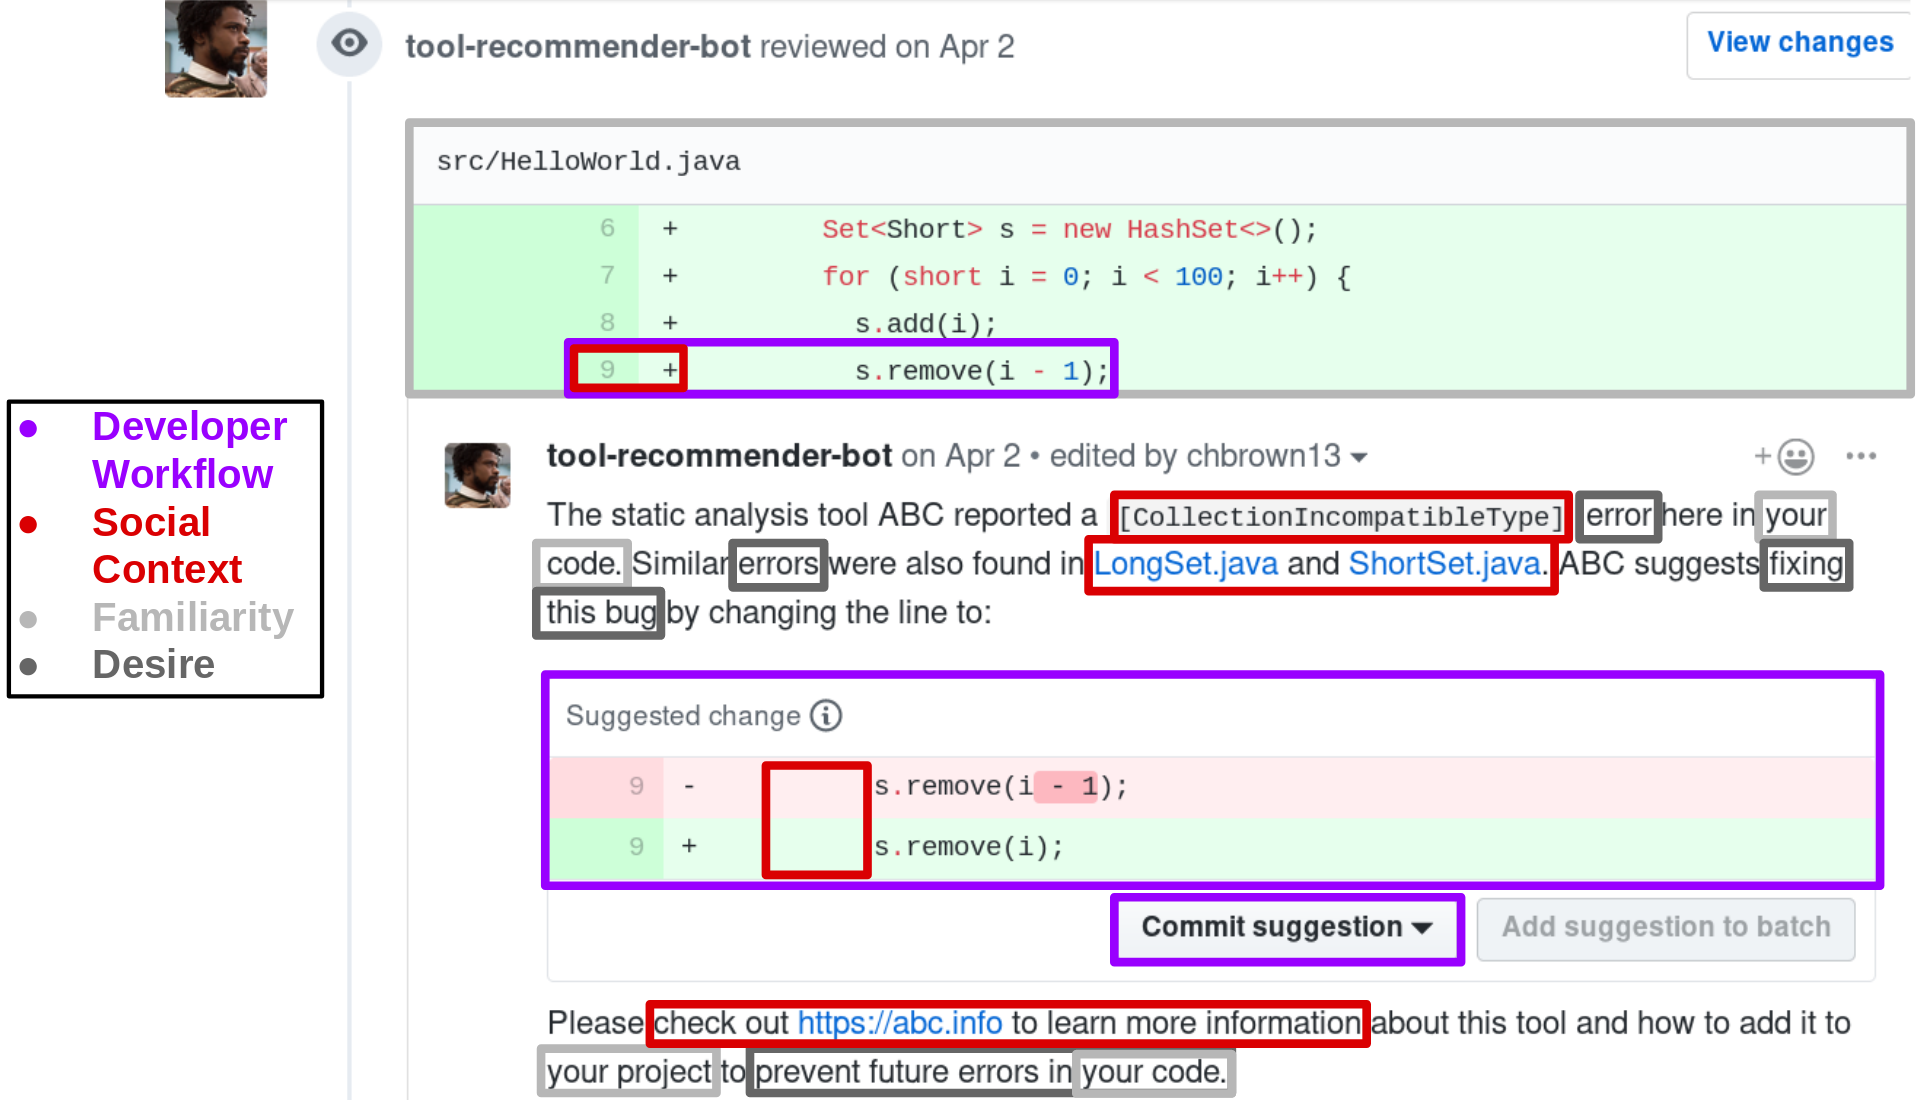
\includegraphics[width=\textwidth]{images/toolapproach.png}
% 	\caption{Prototype implementation of the framework in \TOOL}	
% 	\label{fig:approach} 
% \end{figure*}


% We iteratively modified \TOOL to use different recommendation approaches for nudging developers to adopt different software engineering tools. \TOOL uses a human-presenting GitHub account to recommend tools to developers. , and we also quickly discovered bot accounts are ineffective for recommendations after our original \TOOL~user\footnote{https://github.com/tool-recommender-bot} was flagged and disabled on GitHub for ``opening multiple unsolicited pull requests in other users' repositories" within a few hours of making recommendations at the beginning of our \tele~study. Our goal is for \TOOL~to integrate numerous recommendation approaches and make software engineering tool recommendations using the most effective nudge type(s) when developers are most receptive to adoption.

%\subsubsection{Spatial.}

%Nudge theory suggests that the placement of options in choice environments, or spatial locality, is an important factor in impacting human behavior and decision-making. For example, the director of food services for a school system with hundreds of thousands of children was able to convince students to eat healthier foods and less junk food by simply changing the arrangement of food choices in the cafeteria, i.e. placing carrots at eye-level instead of French fries. Using this strategy, the director was able to nudge students to adopt better diets and change the consumption of specific food items by up to 25\%~\cite[p.~1]{sunstein2008nudge}. 

%We hypothesize location impacts the effectiveness of recommendations to software engineers. For example, developers are more likely to ignore tool suggestions in emails compared to comments in the code. There are many examples of high spatial locality in software engineering. Most integrated development environments have built-in analyzers that highlight syntax errors at the line of code where developers introduce them. Figure \ref{fig:spatial} shows an example of an error reported by the tool  Pylint\footnote{https://www.pylint.org/}, a static analysis tool for Python. 

%\subsubsection{Temporal.}

%Research in nudge theory also suggests that timing of recommendations, or temporal locality, plays a role in influencing behavior. One instance of this is the concept of temptation, where Sunstein and Thaler categorize ``hot" and ``cold" states and note that humans are more likely to make certain decisions during hot times~\cite[p.~41]{sunstein2008nudge}. For example, a study found that simply asking people if they intend to purchase a new car within the next six months actually increased purchase rates by 35\%~\cite{morwitz1993intent}. \todo{Better example of timing}

%We examine temporal locality to determine if the timing of tool recommendations to software engineers impacts adoption. \todo{SE example}

%\subsection{Actionability}

%Nudge theory also suggests that actionability, or the ease in which humans can adopt decisions, impacts the choices people make.  

%We believe that actionability is another important factor in the outcome of recommendations to software engineers. \todo{SE example}

% \section{Tools}

This section outlines concepts for tools to develop and existing systems to observe for evaluating our approaches in making effective recommendations to software engineers.

\subsection{\TOOL}

% Prior work indicates \textit{active help systems} are more effective for providing suggestions to software users than passive help systems, which require users to deliberately seek help~\cite{FischerActiveHelp}.

% Research shows using software engineering tools can improve the quality of software and the efficiency of developers, but in reality developers rarely use them.

To evaluate approaches for making digital nudges to software engineers for development tool adoption, we developed \TOOL. We aim for researchers to be able to extend \TOOL to recommend useful tools to software engineers. Our system is designed to target developer receptivity in recommendations: the \textit{desire} of programmers to produce high-quality code and their \textit{familiarity} with a project's code base. \TOOL~is an automated recommender system designed to suggest software engineering tools to developers on GitHub\footnote{https://github.com}. We target GitHub users because the code hosting and collaboration website has millions of accounts and public repositories, as well as billions of code contributions from developers\footnote{https://octoverse.github.com/}. \TOOL~recommends development tools by integrating with projects' build configuration. With the rise of continuous integration and deployment, many projects implement build systems to automatically compile, test, and release their software more efficiently~\cite{AkondDeployment}. Integrating projects into the build allows developers to easily integrate new tools into their normal software development workflow. We iteratively modified \TOOL to use different recommendation approaches for nudging developers to adopt different software engineering tools. \TOOL uses a human-presenting GitHub account to recommend tools to developers. Prior work found that bots emulating humans are more effective than bot accounts~\cite{AmongTheMachines}, and we also quickly discovered bot accounts are ineffective for recommendations after our original \TOOL~user\footnote{https://github.com/tool-recommender-bot} was flagged and disabled on GitHub for ``opening multiple unsolicited pull requests in other users' repositories" within a few hours of making recommendations at the beginning of our \tele~study. Our goal is for \TOOL~to integrate numerous recommendation approaches and make software engineering tool recommendations using the most effective nudge type(s) when developers are most receptive to adoption.

\subsection{\SUGGS}

GitHub recently introduced a new feature that allows developers to suggest a change to a project's code modified by a user.\footnote{https://help.github.com/articles/incorporating-feedback-in-your-pull-request/\#applying-a-suggested-change} Suggestions can be utilized during pull request reviews, allowing reviewers to propose changes at the exact line of code in question and developers to easily accept or reject the change. Code reviews are another example of a software engineering action shown to improve code quality, and early feedback on the suggestion feature shows they are very popular and widely adopted by GitHub users. We plan to evaluate the effectiveness of GitHub suggestions as examples of a \location. These situated nudges already have over 100,000 uses on GitHub projects and developers are ``quick to adopt suggested changes" and integrate this feature into their code review process.\footnote{https://blog.github.com/2018-11-01-suggested-changes-update/} This research aims to examine situated nudges in the context of \SUGGS~to determine if the location of recommendations impacts the effectiveness of adoption for developers.

\subsection{nudge-bot}

